% Copyright (C) 2012 Shi.Zhan <g.shizhan.g@gmail.com>
%
% Permission is hereby granted, free of charge, to any person obtaining a copy of this software and associated documentation files (the "Software"), to deal in the Software without restriction, including without limitation the rights to use, copy, modify, merge, publish, distribute, sublicense, and/or sell copies of the Software, and to permit persons to whom the Software is furnished to do so, subject to the following conditions:
%
% The above copyright notice and this permission notice shall be included in all copies or substantial portions of the Software.
%
% THE SOFTWARE IS PROVIDED "AS IS", WITHOUT WARRANTY OF ANY KIND, EXPRESS OR IMPLIED, INCLUDING BUT NOT LIMITED TO THE WARRANTIES OF MERCHANTABILITY, FITNESS FOR A PARTICULAR PURPOSE AND NONINFRINGEMENT. IN NO EVENT SHALL THE AUTHORS OR COPYRIGHT HOLDERS BE LIABLE FOR ANY CLAIM, DAMAGES OR OTHER LIABILITY, WHETHER IN AN ACTION OF CONTRACT, TORT OR OTHERWISE, ARISING FROM, OUT OF OR IN CONNECTION WITH THE SOFTWARE OR THE USE OR OTHER DEALINGS IN THE SOFTWARE.
%
% 课程:人机交互技术及应用
% 班级:传播学1001班
% 课时:40学时,2012年秋季1~10周,每周一、三
% 地点:东九楼D212
% 主页:http://code.google.com/p/hci-course/
% 教师:施展 
% 单位:华中科技大学 武汉光电国家实验室
%
\documentclass{beamer}
\usepackage{fontspec,xunicode,xltxtra,beamerthemesplit}
%\usetheme{Hannover} % White background
\usetheme{Berkeley} % Blue background
\setsansfont[Mapping=tex-text, ItalicFont={Courier Italic}]{Microsoft YaHei}

% 中文环境自动换行
\XeTeXlinebreaklocale "zh"
\XeTeXlinebreakskip = 0pt plus 1pt

% 中文环境修正导航栏
\makeatletter
\def\beamer@linkspace#1{
	\begin{pgfpicture}{0pt}{-1.5pt}{#1}{5.5pt}
		\pgfsetfillopacity{0}
		\pgftext[x=0pt,y=-1.5pt]{.}
		\pgftext[x=#1,y=5.5pt]{.}
	\end{pgfpicture}
}
\makeatother

% diagrams
\usepackage{tikz}

\tikzset{
	every overlay node/.style={
		anchor=north west,
	},
}
% Usage:
% \tikzoverlay at (-1cm,-5cm) {content};
% or
% \tikzoverlay[text width=5cm] at (-1cm,-5cm) {content};
\def\tikzoverlay{%
	\tikz[baseline,overlay]\node[every overlay node]
}%

\title{人机交互技术}
\author{施展}
\institute{华中科技大学~武汉光电国家实验室}
\date{\today}
\titlegraphic{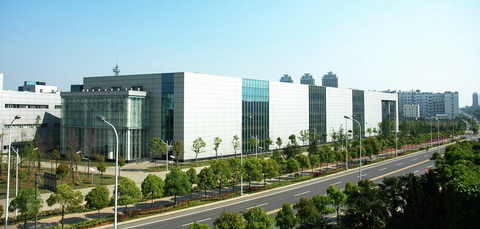
\includegraphics[width=2cm]{images/wnlo.jpg}}

\begin{document}

\begin{frame}
	\titlepage
\end{frame}

\begin{frame}
	\frametitle{内容提要}
	\tableofcontents
\end{frame}

\section{第三讲}
\begin{frame}
	\frametitle{第三讲 交互设备}
	\begin{itemize}
%		\item 了解文本输入设备,图像输入设备,指点输入设备,掌握三维图形输入设备
		\item 了解文本输入设备,图像输入设备,触摸屏输入设备,体感输入设备
%		\item 了解显示器,声音的输出,数字纸等输出设备
		\item 了解显示器,声音的输出,电子墨水等输出设备
%		\item 了解虚拟现实交互设备
	\end{itemize}
\end{frame}

\subsection{输入设备}
\begin{frame}
	\frametitle{输入设备}
	\begin{center}
	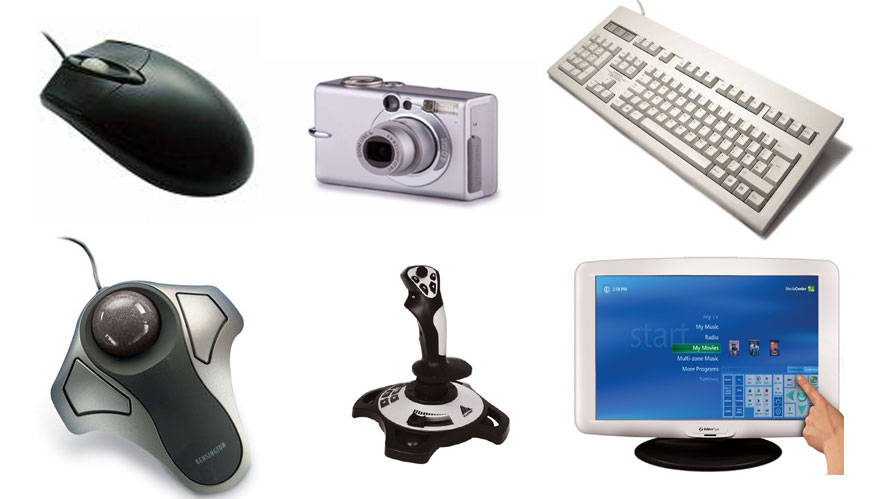
\includegraphics[width=\textwidth]{images/input-devices.jpg}
	\end{center}
\end{frame}

\subsubsection{文本输入设备}
\begin{frame}
	\frametitle{文本输入设备}
	\begin{itemize}
		\item 文本输入是人与计算机交互的一个重要组成部分,同时也是一项繁重的工作。
		\begin{itemize}
			\item 键盘为主
			\item 手写、识别(字符/条码、图像、语音)为辅
		\end{itemize}
	\end{itemize}
\end{frame}

\begin{frame}
	\label{lecture03:keyboard}
	\frametitle{键盘 Keyboard}
	\transglitter % Glitter sweeps in specified direction
	\transduration<1,2,3>{.2} % Show slide specified number of seconds
	\tikzoverlay at (0cm,-3cm) {文本输入最主要手段~{\tiny 应用环境影响布局,布局影响速度、准确性、舒适度。}};\pause
	\tikzoverlay at (3cm, 4.5cm) {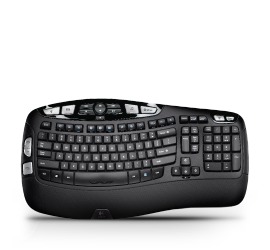
\includegraphics[width=5cm]{images/keyboard.png}};\pause
	\tikzoverlay at (0cm, 0cm) {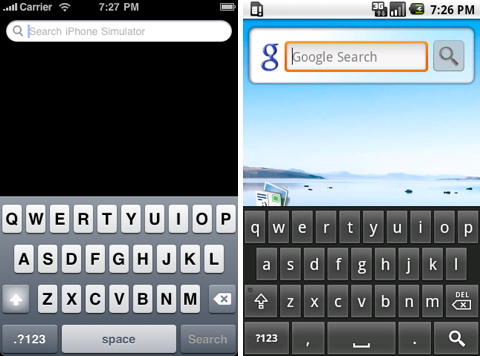
\includegraphics[width=3cm]{images/mobile_keyboards.png}};\pause
	\tikzoverlay at (6cm, 0cm) {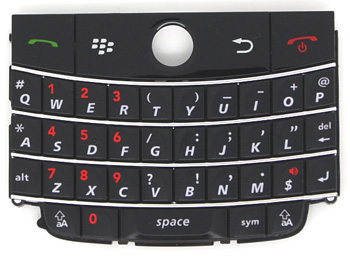
\includegraphics[width=3cm]{images/blackberry-bold-9000-keyboard.jpg}};
\end{frame}

\begin{frame}
	\frametitle{键盘分类}
	\beamertemplatetransparentcovereddynamicmedium
	\begin{itemize}
		\item 编码键盘
		\begin{itemize}
			\item 控制电路的功能完全依靠硬件自动完成,能自动将所按下的按键的编码信息送入计算机。
			\item 响应速度快,但硬件结构复杂。
		\end{itemize}\pause
		\item 非编码键盘
		\begin{itemize}
			\item 控制电路功能要依靠硬件和软件共同完成。
			\item 虽然响应速度不如编码键盘快,但可通过软件为键盘的某些按键重新定义,容易扩充键盘功能,应用广泛。
		\end{itemize}
	\end{itemize}
\end{frame}

\begin{frame}
	\frametitle{键盘布局}
	\begin{itemize}
		\item QWERTY键盘布局
		\begin{itemize}
			\item 19世纪70年代,Christopher Sholes发明了QWERTY键盘布局,其名称来源于该布局方式最上行前6个英文字母,最常用的几个字母安置在相反方向,最大限度放慢敲键速度以避免卡键。
			\item 这种布局方式依然是今天最为常见的排列方式{\tiny (第\ref{lecture03:keyboard}页)},成为一种事实上的标准。
		\end{itemize}
	\end{itemize}
	\begin{center}
	% http://zh.wikipedia.org/wiki/QWERTY鍵盤
	% http://upload.wikimedia.org/wikipedia/commons/3/3a/Qwerty.svg
	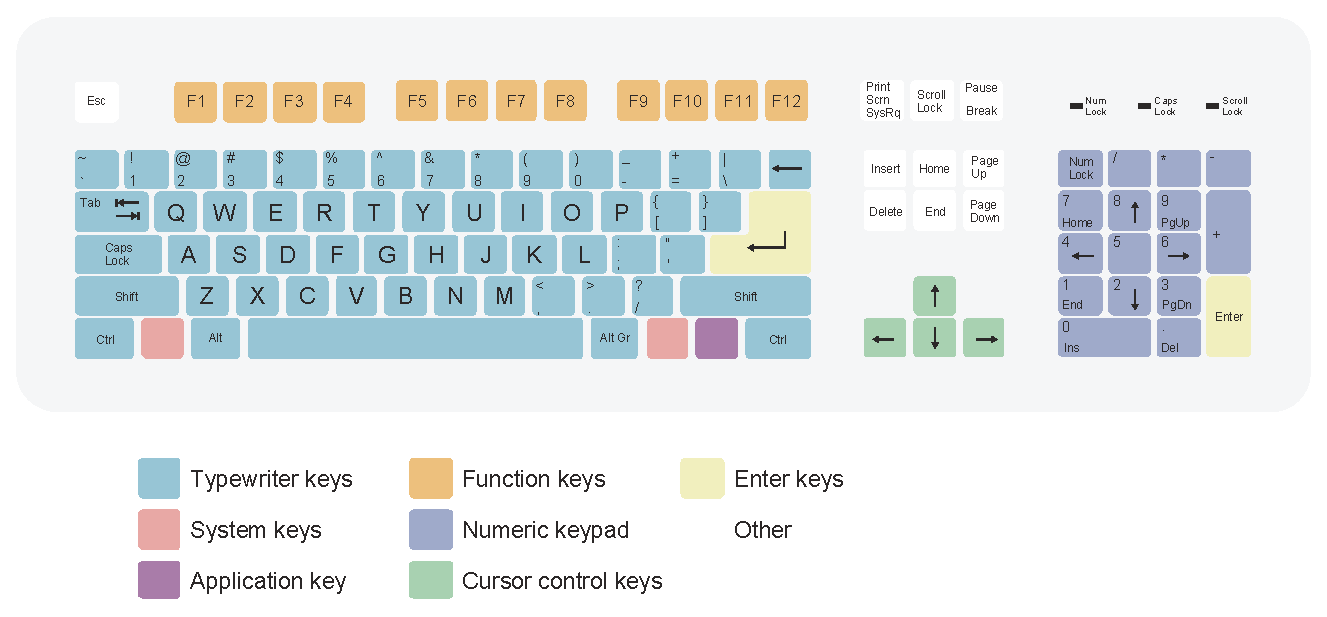
\includegraphics[width=8cm]{images/qwerty.eps}
	\end{center}
\end{frame}

\begin{frame}
	\frametitle{键盘布局}
	\begin{itemize}
		\item DVORAK键盘布局
		% http://www.cnbeta.com/articles/120272.htm
		% http://baike.baidu.com/view/1410112.htm
		\begin{itemize}
			\item 20世纪20年代的DVORAK键盘布局,据推测使用DVORAK,打字者的手指平均每日运动1英里,而QWERTY则是12到20英里。
			\item DVORAK可以大大减少手指移动距离,从而大大提高输入速度,但由于受到传统QWERTY布局的影响,没有成为主流的键盘布局。
		\end{itemize}
	\end{itemize}
	\begin{center}
	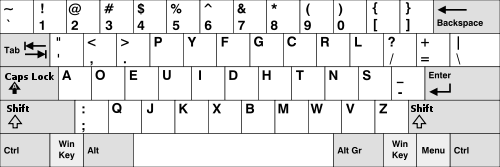
\includegraphics[width=8cm]{images/dvorak.png}
	\end{center}
\end{frame}

\begin{frame}
	\frametitle{人机工程学键盘 Ergonomic Keyboard}
	%\beamertemplatetransparentcovereddynamicmedium
	\transdissolve
	% the above can't be used since it will prevent the picture to show correctly
	% http://www.hudong.com/wiki/人体工学键盘
	% http://www.osha.gov/SLTC/etools/computerworkstations/components_keyboards.html
	% http://www.ergonomics-info.com/computer-ergonomic-keyboard.html
	\begin{center}
		\onslide<1->{
			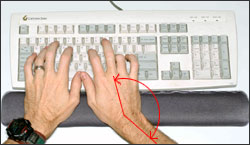
\includegraphics[width=3cm]{images/comp_keyboard_angledwrist.jpg}~
			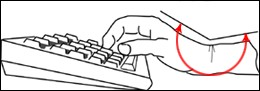
\includegraphics[width=4cm]{images/comp_keyboard_bent_wrist.jpg}\\
			{\tiny 长时间悬腕或塌腕将造成关节劳累——腕管综合征}\\
		}
		\onslide<2->{
			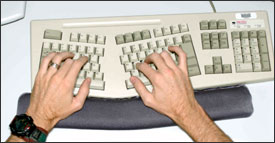
\includegraphics[width=3cm]{images/comp_keyboard_ergo.jpg}~
			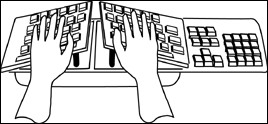
\includegraphics[width=4cm]{images/comp_keyboard_tented.jpg}\\
			{\tiny 将两手所控的键位向两旁分开一定的角度,使两臂自然分开,缓解臂、腕疲劳}\\
		}
		\onslide<3->{
			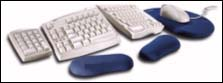
\includegraphics[width=4cm]{images/alternative_keyboard.jpg}~
			{\tiny 增加腕托}
		}
	\end{center}
\end{frame}

\begin{frame}
	\frametitle{人机工程学键盘 Ergonomic Keyboard}
	\transdissolve
	\begin{itemize}
		\onslide<1->{\item 目前这类键盘品种很多,有固定式、分体式和可调角度式,以适应不同操作者的各种姿势。}
		\onslide<2->{
			\item 微软自然键盘 Microsoft Nature Keyboard\\
			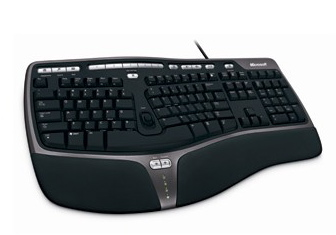
\includegraphics[width=4cm]{images/microsoft-natural-ergonomic-keyboard-4000.jpg}~
			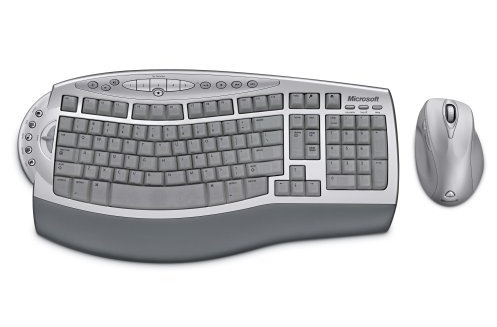
\includegraphics[width=4cm]{images/ergonomic-keyboard-mac-microsoft.jpg}
		}
	\end{itemize}
\end{frame}

\begin{frame}
	\frametitle{人机工程学键盘 Ergonomic Keyboard}
	\transdissolve
	\begin{itemize}
		\item 目前这类键盘品种很多,有固定式、分体式和可调角度式,以适应不同操作者的各种姿势。
		\item Kinsis, Logitec 人体工学键盘 \dots\\
		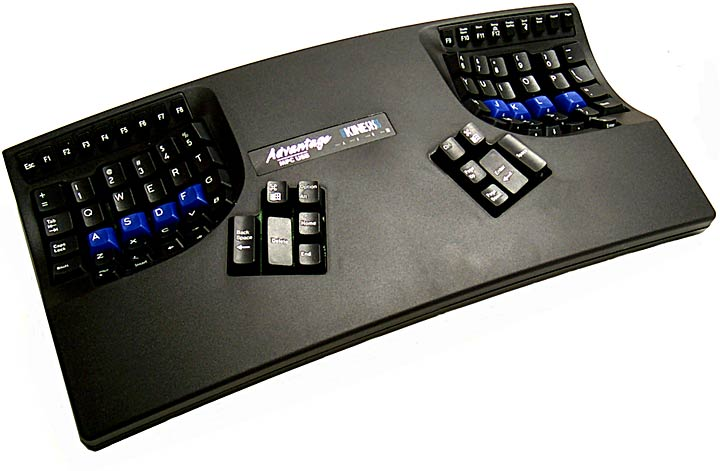
\includegraphics[width=4cm]{images/kinesis-advantage-keyboard.jpg}~
		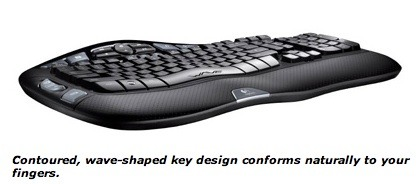
\includegraphics[width=4cm]{images/logitech-ergonomic-keyboard-wave.jpg}
	\end{itemize}
\end{frame}

\begin{frame}
	\frametitle{人机工程学键盘 Ergonomic Keyboard}
	\transdissolve
	\begin{itemize}
		\item 目前这类键盘品种很多,有固定式、分体式和可调角度式,以适应不同操作者的各种姿势。
		\item 分体式人体工学键盘 Modular Ergonomic Keyboard\\
		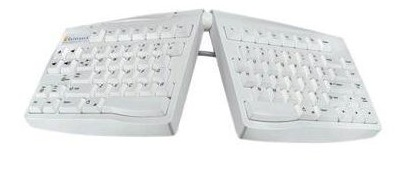
\includegraphics[width=4cm]{images/ergonomic-keyboard-mac-goldtouch.jpg}~
		% http://elecinlife.com/modular-ergonomic-keyboard-falls-to-pieces/
		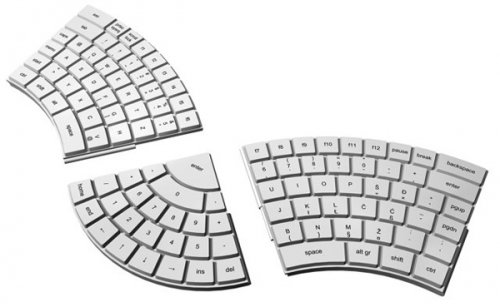
\includegraphics[width=4cm]{images/ergonomic-modular-keyboard-falls-to-pieces_1.jpg}\\
		\begin{center}
		% http://c2.com/cgi/wiki?KinesisEvolutionKeyboard
		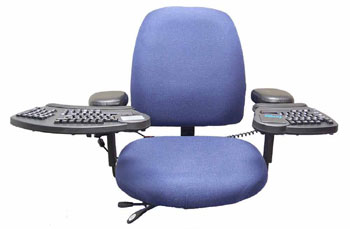
\includegraphics[width=4cm]{images/keyboard-chair.jpg}
		\end{center}
	\end{itemize}
\end{frame}

\begin{frame}
	\frametitle{多功能集成键盘}
	\transdissolve
	\begin{itemize}
		\item 游戏、无线、DJ\\
		% http://www.coolest-gadgets.com/20071120/hybrid-gaming-keyboard-gives-you-all-the-keys-you-need-but-you-still-cant-type-well-on-it/
		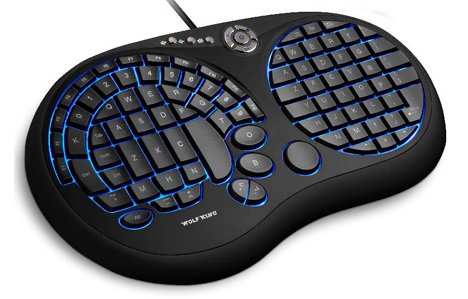
\includegraphics[width=4cm]{images/wolfking-warrior-xxtreme.jpg}~
		% http://achknowledge.wordpress.com/2011/06/23/best-gaming-keyboard-and-mouse/
		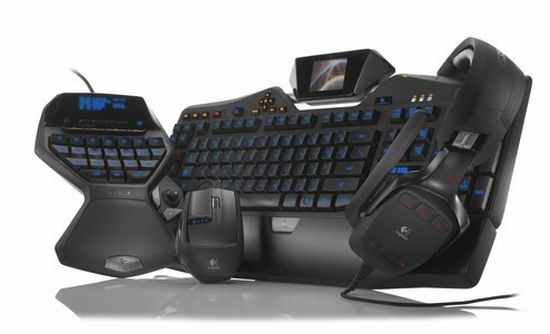
\includegraphics[width=4cm]{images/logitech-g19-gaming-keyboard.jpg}\\
		% http://www.walmart.com/ip/The-Singing-Machine-Sound-X-Kids-Electronic-Keyboard-DJ-Mixer/17133266
		\begin{center}
		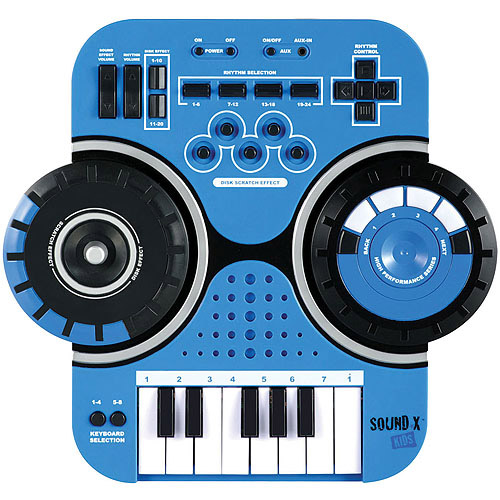
\includegraphics[width=3cm]{images/sound-x-electronic-keyboard-dj-mixer.jpg}
		\end{center}
	\end{itemize}
\end{frame}

\begin{frame}
	\frametitle{手写设备}
	\begin{itemize}
		\item 手写板+手写笔
		\item {\tiny 除用于文字、符号、图形等输入外,还可提供光标定位功能,从而同时替代键盘与鼠标}
	\end{itemize}
	% http://m.pconline.com.cn/shop123090/nid:3118168/news_detail.html
	\begin{center}
		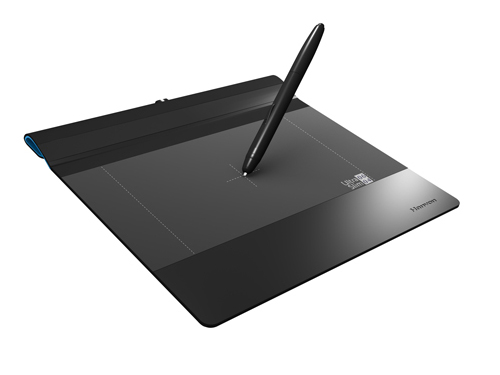
\includegraphics[width=4cm]{images/drawing-pad-hanwang.jpg}~
		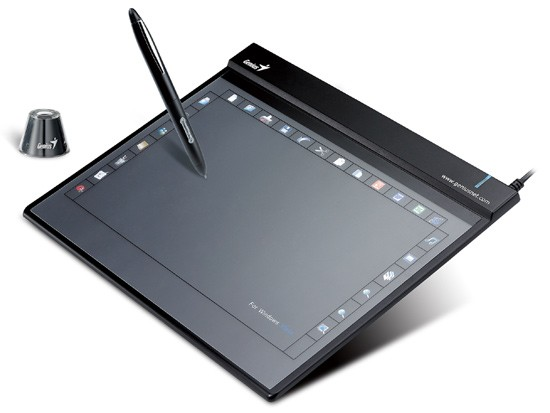
\includegraphics[width=4cm]{images/drawing-pad-mengtian.jpg}
	\end{center}
\end{frame}

\begin{frame}
	\frametitle{手写板}
	% http://baike.baidu.com/view/207382.htm
	\begin{itemize}
		\item 电阻式压力手写板:几乎已经被淘汰
		\item 电磁式感应手写板:目前市场主流产品
		\item 电容式触控手写板:市场的新生力量,具有耐磨损、使用简便、敏感度高等优点,是今后手写板的发展趋势。
	\end{itemize}
\end{frame}

\begin{frame}
	\frametitle{光学字符识别 Optical Character Recognition}
	\beamertemplatetransparentcovereddynamicmedium
	% http://baike.baidu.com/view/17761.htm
	\begin{itemize}[<+->]
		\item 对文本资料的图像文件进行分析处理,获取文字及版面信息的过程。
		\item 在1929年由德国科学家Tausheck最先提出来的,后来美国科学家Handel也提出了利用技术对文字进行识别的想法。
		\item 最早对印刷体汉字识别进行研究的是IBM公司的Casey和Nagy,1966年他们发表了第一篇关于汉字识别的文章,采用了模板匹配法识别了1000个印刷体汉字。
		\item 20世纪70年代初,日本的学者开始研究汉字识别,并做了大量的工作。
		\item 中国在OCR技术方面的研究工作起步较晚,70年代末开始进行汉字识别的研究,80年代产品化。
	\end{itemize}
\end{frame}

\begin{frame}
	\frametitle{光学字符识别 Optical Character Recognition}
%图像处理模块
%版面划分模块 
%文字识别模块 
%文字编辑模块
%
%影像输入、影像前处理、文字特征抽取、比对识别、人工校正、结果输出
\end{frame}

\begin{frame}
	\frametitle{手写汉字识别 Handwriting Recognition}

\end{frame}

\subsubsection{指点输入设备}
\begin{frame}
	\frametitle{指点输入设备}
	\begin{itemize}
		\item 指点设备常用于完成一些定位和选择物体的交互任务。
		\item 物体可能处于一维、二维、三维或更高维的空间中。
		\item 选择与定位的方式可以是直接选择,或通过操作屏幕上的光标来完成。
	\end{itemize}
\end{frame}

\begin{frame}
	\frametitle{鼠标 Mouse}

\end{frame}

\begin{frame}
	\frametitle{鼠标的分类}

\end{frame}

\begin{frame}
	\frametitle{鼠标与计算机的接口}

\end{frame}

\begin{frame}
	\frametitle{鼠标的结构}

\end{frame}

\begin{frame}
	\frametitle{新型鼠标}

\end{frame}

\begin{frame}
	\frametitle{触摸板 Touchpad}

\end{frame}

\begin{frame}
	\frametitle{控制杆 Joy Stick}

\end{frame}

\begin{frame}
	\frametitle{触摸屏 Touch Screen}

\end{frame}

\begin{frame}
	\frametitle{触摸屏的组成与分类}

\end{frame}

\begin{frame}
	\frametitle{多点触摸}

\end{frame}

\subsubsection{图像输入设备}
\begin{frame}
	\frametitle{图像输入设备}

\end{frame}

\begin{frame}
	\frametitle{扫描仪}

\end{frame}

\begin{frame}
	\frametitle{数码摄像头}

\end{frame}

\subsection{输出设备}
\begin{frame}
	\frametitle{输出设备}

\end{frame}

\subsubsection{显示器}
\begin{frame}
	\frametitle{显示器}

\end{frame}

\subsubsection{打印机}
\begin{frame}
	\frametitle{打印机}

\end{frame}

\subsubsection{电子墨}
\begin{frame}
	\frametitle{电子墨}

\end{frame}

\subsubsection{语音交互设备}
\begin{frame}
	\frametitle{语音交互设备}

\end{frame}

\section{小结}
\begin{frame}
	\frametitle{小结}
	\begin{itemize}
		\item 输入设备:
		\begin{itemize}
			\item 文本输入设备
			\item 图像输入设备
			\item 指点输入设备\dots
		\end{itemize}
		\item 输出设备:
		\begin{itemize}
			\item 显示器 
			\item 打印机
			\item 声音的输出\dots
		\end{itemize}
	\end{itemize}
\end{frame}
 
\begin{frame}
	\frametitle{参考文献}
	\bibliographystyle{plain}
	\bibliography{hci}
\end{frame}

\end{document}